% Gerado de tcc.md (exportado do Claude Docs) por ferramentas/gera_latex.php em 12/11/2026 21:45.
% Para mudar o texto, edite este arquivo; se gerar de novo a partir do documento, as edições feitas aqui se perdem.

\chapter{INTRODUÇÃO}\label{cap:1}

A educação especial cresceu de forma contínua na última década. O Gráfico~\ref{graf:1} mostra o número de matrículas dessa modalidade nos dez últimos Censos Escolares da Educação Básica, de 2016 a 2025, com os valores das notas estatísticas publicadas pelo Instituto Nacional de Estudos e Pesquisas Educacionais Anísio Teixeira (INEP).

\begin{grafico}[hbp]
  \legendafig{grafico}{Matrículas na educação especial no Brasil, 2016-2025}{graf:1}
  % Gráfico de linhas das matrículas na educação especial no Brasil de 2016 a 2025, em milhares: 971,4 em 2016, 1.066,4 em 2017, 1.181,3 em 2018, 1.251,0 em 2019, 1.308,9 em 2020, 1.350,9 em 2021, 1.527,8 em 2022, 1.771,4 em 2023, 2.076,8 em 2024 e 2.458,2 em 2025
  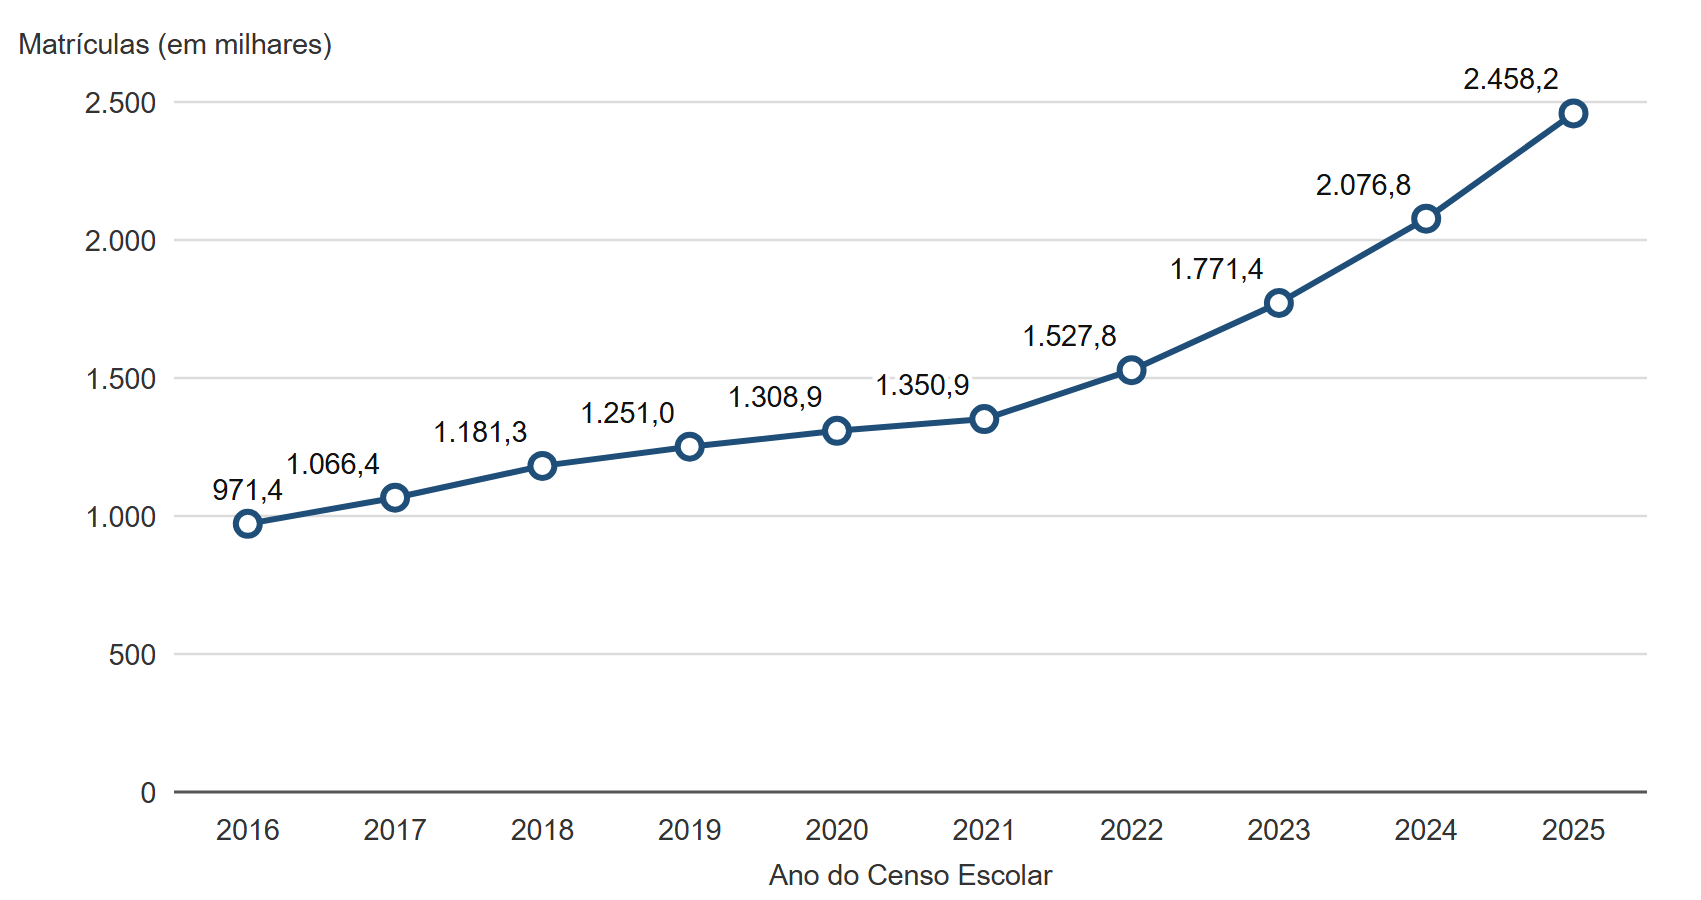
\includegraphics[width=15cm,height=17cm,keepaspectratio]{figuras/grafico01-censo.png}
  \fonte{elaborado pelo autor com base em INEP (2021, p. 22; 2026, p. 24).}
\end{grafico}

Entre 2016 e 2025, as matrículas na educação especial passaram de 971.372 para 2.458.159, um aumento de 153\%. O crescimento acelerou nos últimos anos: de 2016 a 2021, o número subiu 39\%; de 2021 a 2025, subiu 82\%, cerca de 1,1 milhão de matrículas a mais em quatro anos. No mesmo período, a parcela de estudantes de 4 a 17 anos da educação especial incluídos em classes comuns passou de 93,5\% para 96,0\% (INEP, 2026, p. 24). Mais estudantes da educação especial nas classes comuns significa mais planos individualizados para elaborar e, principalmente, para acompanhar, o que aumenta a necessidade de ferramentas que apoiem o professor nesse trabalho.

Os valores de 2016 a 2020 vêm das notas estatísticas do Censo de 2020 (INEP, 2021, p. 22), e os de 2021 a 2025, das notas do Censo de 2025 (INEP, 2026, p. 24). A série de matrículas é comparável: a edição intermediária de 2024 repete os mesmos totais, como os 1.308.900 de 2020 (INEP, 2025, p. 20). O percentual em classes comuns, ao contrário, foi revisado entre edições, com 93,3\% para 2020 na edição de 2021 e 93,2\% na de 2025, e por isso é citado aqui apenas para 2021 a 2025, a partir de uma única edição.

Estar matriculado na classe comum não garante aprendizagem. Para isso, a escola precisa planejar o ensino a partir do que cada estudante já sabe e do que precisa aprender. O Plano Educacional Individualizado (PEI) é o instrumento desse planejamento. Tannús-Valadão e Mendes (2018, p. 11) apontam, entre as funções do PEI, a de registro dos conhecimentos e das habilidades do aluno, “que permite identificar o repertório de partida, acompanhar a evolução em direção às metas e traçar novos caminhos, se determinado programa não estiver permitindo atingir as metas estabelecidas para o estudante”. Com o Decreto nº 12.686/2025, que instituiu a Política Nacional de Educação Especial Inclusiva, e a alteração feita pelo Decreto nº 12.773/2025, passou a ser obrigatório um “documento individualizado de natureza pedagógica, com atualização contínua”, como o Plano de Atendimento Educacional Especializado (PAEE) e o PEI, derivado do estudo de caso do estudante (BRASIL, 2025a, art. 12).

A expressão “atualização contínua” expõe o ponto mais frágil do PEI: o acompanhamento. Tannús-Valadão e Mendes (2018, p. 1, 11-12) relatam um levantamento anterior, feito por Tannús-Valadão em 200 planos de Atendimento Educacional Especializado (AEE) de um município paulista, cujo preenchimento parecia ser feito “por mera formalidade”, com repetições, incoerências e plano formalizado para apenas um terço dos alunos; ao comparar o Brasil com outros países, as autoras concluem que, embora se anuncie a inclusão escolar, “as práticas de planejamento não mudaram”. Sem registros frequentes do desempenho, a revisão do plano depende da memória do professor e de impressões gerais, o que torna difícil dizer se uma meta foi alcançada ou se a estratégia precisa mudar.

Em sua dissertação de mestrado, a pesquisadora Priscila Rodrigues Cruz Francisco enfrentou parte desse problema com o AppPEI (FRANCISCO, 2023), um recurso educacional digital construído em planilha eletrônica, que conduz o professor pelas etapas de elaboração do PEI: dados do aluno, avaliação diagnóstica, matriz de habilidades em quatro áreas, priorização e proposta de intervenção. Na avaliação feita com professores do Colégio de Aplicação da Universidade do Estado do Rio de Janeiro (UERJ), 75\% dos respondentes consideraram o recurso intuitivo, a nota média foi 8,25 e os participantes sugeriram trocar a planilha por uma página web, com navegação mais simples e uso no celular (FRANCISCO, 2023). O AppPEI organiza o planejamento, mas não mede o desempenho do aluno nas habilidades planejadas; a verificação da evolução continua fora da ferramenta.

Este trabalho apresenta o UNIA (Unir Necessidades Individuais e Aprendizagem), um sistema web que parte da estrutura do AppPEI e acrescenta a medição. O nome também remete ao verbo unir: o sistema une as metas do PEI, definidas a partir das necessidades de cada aluno, à medição da aprendizagem nas sessões. O professor cadastra o aluno, o estudo de caso e as metas do PEI; o aluno responde a mini games na tela; o sistema confere cada resposta, classifica o nível de suporte de cada sessão com os mesmos três níveis do AppPEI e mostra a evolução de cada meta em indicadores e gráficos. A revisão do plano passa a contar com uma série de sessões medidas, e não só com a impressão de quem acompanha o aluno.

A pergunta que orienta o trabalho é: como um sistema web pode apoiar o professor no acompanhamento das metas do PEI, medindo de forma automática o desempenho do aluno em atividades digitais e mostrando a evolução ao longo do tempo?

\section{Justificativa}\label{sec:1.1}

A primeira razão é normativa. A Resolução nº 4/2009 do Conselho Nacional de Educação, Câmara de Educação Básica (CNE/CEB), atribui ao professor do AEE a elaboração e a execução do plano de AEE, avaliando a funcionalidade e a aplicabilidade dos recursos pedagógicos, e o acompanhamento desses recursos na sala de aula comum (BRASIL, 2009, art. 13). A Lei Brasileira de Inclusão inclui, entre os deveres do poder público, o planejamento de estudo de caso, a elaboração de plano de atendimento educacional especializado e a usabilidade pedagógica de recursos de tecnologia assistiva (BRASIL, 2015, art. 28, VII). A norma de 2025 reforça essas atribuições ao exigir atualização contínua do PAEE e do PEI (BRASIL, 2025a, art. 12), e a Portaria nº 421/2026 do Ministério da Educação (MEC), que a regulamenta, inclui entre os conteúdos mínimos do PEI “as estratégias de acompanhamento e de monitoramento do plano” (BRASIL, 2026, art. 11, III). Acompanhar exige registros, e registros feitos à mão a cada sessão consomem um tempo que o professor raramente tem.

A segunda razão é a lacuna nas ferramentas. Francisco (2023) não encontrou aplicativos de PEI na loja Google Play. Nas fontes consultadas nesta pesquisa (seção~\ref{sec:2.5}), as ferramentas digitais tratam ou da elaboração e do registro do PEI ou de jogos para a aprendizagem; não se encontrou uma que associe o desempenho medido nos jogos às metas do plano. Um sistema com essa ligação também atende ao pedido dos professores que avaliaram o AppPEI, que sugeriram um formato web acessível pelo celular.

A terceira razão é pedagógica. O PEI existe para que o aluno avance em direção à autonomia, isto é, para que passe a realizar sozinho o que antes realizava com ajuda. Esse movimento corresponde à passagem entre os níveis “realiza com ajuda” e “realiza sem necessidade de suporte” do AppPEI e, na teoria histórico-cultural, à ideia de que aquilo que a criança faz hoje com assistência ela fará sozinha amanhã (VIGOTSKI, 2007). Tornar essa passagem visível, sessão após sessão, ajuda o professor a decidir quando retirar o apoio e quando mudar a estratégia.

\section{Objetivos}\label{sec:1.2}

\subsection{Objetivo geral}\label{sec:1.2.1}

Desenvolver um sistema web que apoie o professor no acompanhamento das metas do PEI de alunos da educação especial dos anos iniciais, medindo de forma automática o desempenho em mini games e apresentando a evolução de cada meta.

\subsection{Objetivos específicos}\label{sec:1.2.2}

\begin{alineasIFTO}
  \item identificar, na legislação e na literatura, os elementos do PEI e os níveis de suporte usados para acompanhar metas, tomando o AppPEI como referência;
  \item modelar e implementar o cadastro de alunos, do estudo de caso e das metas por área, com nível de suporte inicial e data de revisão;
  \item desenvolver mini games que registrem acerto, uso de dica e tempo de resposta nas quatro áreas da matriz do AppPEI;
  \item definir uma regra de classificação do nível de suporte por sessão e indicadores de evolução por meta, apresentados em tabelas e gráficos acessíveis;
  \item verificar o funcionamento e a usabilidade do sistema por meio de testes automatizados, de um teste de ponta a ponta e de uma avaliação heurística.
\end{alineasIFTO}

\section{Estrutura do trabalho}\label{sec:1.3}

Além desta introdução, o trabalho tem cinco capítulos. O capítulo~\ref{cap:2} reúne a fundamentação teórica: a educação especial na perspectiva inclusiva e seu marco legal, o PEI e os níveis de suporte, a medição frequente do progresso, os jogos digitais na educação e os trabalhos relacionados. O capítulo~\ref{cap:3} descreve a metodologia da pesquisa e do desenvolvimento. O capítulo~\ref{cap:4} apresenta o UNIA: requisitos, arquitetura, modelo de dados, mini games, regras de medição, gráficos, segurança e acessibilidade. O capítulo~\ref{cap:5} discute a verificação técnica, compara o UNIA com o AppPEI, relata a avaliação heurística e expõe as limitações. O capítulo~\ref{cap:6} traz as considerações finais e os trabalhos futuros.
